\documentclass[]{IEEEphot}
\usepackage[utf8]{inputenc}
\usepackage{dtk-logos} % for BibTeX stylized logo

\title{Universisdade Federal do Pará\\Programa de Pós-Graduação em Engenharia Elétrica\\Plano de Trabalho – Mestrado}


\begin{document}

\author{Fernanda Alves Magno}

\affil{Área de Concentração: Sistemas de Energia\\Linha de Pesquisa: Sistemas Elétricos de Potência}  

\maketitle

%\markboth{}{}

%\begin{abstract}
%	O uso de Geração Distribuída traz diversos benefícios. A inserção dessas novas fontes é crescente no mercado. Essa proposta apresenta o projeto da estrutura de uma Microrrede, em uma rede real, inserindo pontos de fontes renováveis e armazenamento de energia. 
%\end{abstract}

%\begin{IEEEkeywords}
%	Dimensionamento Ótimo, Energia Fotovoltaica, Geração Distribuída, Microrrede.
%\end{IEEEkeywords}

	\section{Tema}
Proposta de Controle Volt/Var para Sistemas de Distribuição em \textit{Smart Grids}.

\section{Palavras-chave}
Controle Volt/Var, Fluxo de Potência Ótimo, Operação de Sistemas de Distribuição de Energia Elétrica, \textit{Smart Grids}.

\section{Introdução}
Diante da modernização do Sistema Elétrico de Potência (SEP) com Redes Elétricas Inteligentes (SD do inglês, \textit{Smart Grids}), com a penetração de Recursos Energéticos Distribuídos (DER do inglês, \textit{Distributed Energy Resources}) e de Veículos Elétricos (VEs), é necessário a utilização de técnicas mais adequadas para o controle da tensão e da potência reativa na rede \cite{Agostinho2019}. No Brasil, as regras que classificam a tensão em adequada, precária e crítica são estabelecidas no módulo 8 do PRODIST (Procedimentos de Distribuição) formulado pela Agência Nacional de Energia Elétrica (ANEEL) \cite{M8Prodist}.\\
A modernização ocasionada pelas SG, como o uso de sensores, comunicação e controles inteligentes permite que o estado da rede elétrica seja observado por completo e impulsiona o desenvolvimento de novas técnicas de solução para inúmeras aplicações de auxílio à tomada de decisão, sendo uma destas aplicações o Controle Volt/VAr (VVC do inglês, \textit{Volt/Var Control}) \cite{Mello2018}.\\
Neste sentido, esse plano de trabalho apresenta a proposta de desenvolvimento de um novo método VVC que possibilite o ajuste ótimo dos equipamentos controláveis da rede visando a minimização das perdas de energia e a melhora do perfil de tenção do sistema. O método de solução proposto faz uso da metaheurística Otimização por Enxame de Partículas (PSO do inglês, \textit{Particle Swarm Optimization}). As principais contribuição do trabalho incluem: (I) Algoritmo de VVC coordenado, baseado na efetividade e disponibilidade de equipamentos; (II) Desenvolvimento e implementação de um algoritmo de controle adaptável para distintos objetivos de operação nas redes de distribuição. 
 
%Diversos estudos demonstram o impacto do uso de combustíveis fósseis no meio ambiente. Somado à crescente demanda energética, a necessidade de energia proveniente de fontes não poluentes se torna evidente. Partindo desse ponto de vista, o projeto de geração próximas aos centros de consumo a partir de fontes renováveis é um modo de mitigar esses problemas. O conceito clássico de rede elétrica, onde o fluxo de energia é unidirecional, está sendo alterado devido a principalmente três fatores: integração em larga escala de geradores de energia renováveis, desenvolvimento de novas tecnologias de geração e armazenamento de energia próximo ao local de consumo e a adoção de sistemas de controle e comunicação da rede \cite{Pfitscher2013}.\\
%Essas mudanças têm como objetivos proporcionar a descarbonização da matriz energética, tornando o sistema sustentável, além de tornar a rede mais confiável, estável e eficiente. Todas essas transformações no sistema de energia constituem parte do conceito de Microrredes (MR), que é definido como um sistema elétrico composto por pequenas unidades geradoras, de até algumas centenas de kW, conectados a um barramento de baixa tensão, criando um sistema localmente controlado, que pode ser integrado a rede elétrica principal ou operar de maneira isolada durante desligamentos ou blecautes.
\section{Justificativa}

Equipamentos como transformador com comutação sob carga (LTC), reguladores de tensão e bancos de capacitores foram desenvolvidos e aprimorados para atender com segurança e eficiência a disponibilidade de energia das redes de distribuição e manter a tensão dentro de limites aceitáveis. Entretanto, esta tarefa tem se tornado cada vez
mais complexa devido o crescimento acelerado da participação de fontes renováveis de energia, VEs e dispositivos de armazenamento no SEP \cite{Mercer2016}. Isto tem atraído a atenção de pesquisadores da área, uma vez que esses novos elementos provocam variação de tenção e injeção ou absorção de potência reativa na rede, porém atualmente os sistemas de distribuição possuem uma infraestrutura de controle e medição limitada \cite{Mello2018}.\\
No entanto, os avanços tecnológicos, caracterizados pela aplicação de SD, está mudando este cenário possibilitando o controle e otimização online do perfil de tensão e de potência reativa, visando a melhoria contínua da qualidade de energia, a partir da redução de perdas técnicas, da manutenção da tensão dada a ocorrência de defeito/rejeição de carga na rede, além do uso generalizado de sistemas de geração distribuída (GD).\\
A realização do VVC, a partir dos equipamentos de um sistema de distribuição é essencial para manter a tensão em níveis adequados em todos os pontos do alimentador de distribuição, considerando as mais diversas condições de operação do sistema \cite{Fassbinder2016}. O VVC é uma das funções mais importantes e desejadas no âmbito de sistemas de Automação de Distribuição Avançada (DA) e Sistema de Gerenciamento da Distribuição (DMS do inglês, \textit{Distribution Management System}), o qual tem como uma de suas principais funções a realização de um controle de tensão e potência reativa eficiente e integrado (IVVC, do inglês, \textit{Integrated Volt/Var Control}) \cite{Mercer2016}.\\
A literatura propõem vários métodos e técnicas para a realização do VVC. Métodos como Busca Heurística \cite{Deng2002}, Algoritmo Evolucionário \cite{Ulinuha2008}, \textit{Simulated Annealing} \cite{LiangeWang2003}, Lógica Fuzzy \cite{(LiangeWang2003}, também têm sido utilizados para solução do problema de VVC. Nesta proposta o interesse é a aplicação de métodos metaheurísticos, mais especificadamente, a metaheurística PSO,  para a resolução do Problema de Alocação Ótima entre dispositivos de controle tais como: GDs, reguladores de tensão e bancos de capacitores. Assim como o controle ótimo de Volt/VAr com a presença de GDs apresentado em \cite{Auchariyamet2010}, que tem como objetivo a minimizar é a compra de energia dos GDs e reduzir o custo das perdas de energia durante uma operação diária.\\
A técnica proposta neste plano de trabalho coordena as ações de controle entre os equipamento, considerando os limites físicos e o número de comutações, visando não priorizar um dispositivo específico para atuação no sistema e, consequentemente, preservar a vida útil dos equipamentos utilizados para o controle VVC. Além disso, o método possibilita o uso da comunicação de sistemas supervisórios de equipamentos controlados remotamente.



 
%As MRs têm um papel fundamental no que diz respeito a operação resiliente dos sistemas de energia elétrica, mantendo o atendimento às cargas de maneira confiável e segura, principalmente quando o sistema está sujeito a desastres naturais ou condições climáticas extremas em que ocorrem ilhamento de parte do sistema \cite{Khodaei2014}. É capaz de integrar, controlar e gerir várias fontes de energia, armazenamento e pontos de consumo, além de outros elementos como Veículos Elétricos (VEs), de forma mais eficiente e autônoma. Devido à proximidade entre as fontes geradoras e as cargas atendidas, as MRs apresentam perdas de transmissão reduzidas em comparação aos grandes centros geradores.\\
%Outras vantagens incluem a descentralização da geração de eletricidade, o que aumenta a confiabilidade do fornecimento de energia, e a redução de emissões de gases do efeito estufa \cite{Chowdhury2009}. Essa diminuição de poluentes se dá pelo fato de que fontes não renováveis como geradores a óleo diesel são usadas apenas como último recurso. No geral as MRs são mais confiáveis, sustentáveis, eficientes, têm maior estabilidade e a melhora no perfil de tensão e reduzem as perdas de energia no sistema, além de possibilitar uma economia no consumo de energia proveniente de distribuidoras.\\
%O conceito de produzir energia próximo ao seu local de consumo segue uma tendência de acentuado crescimento nas últimas duas décadas. Essa característica é associada à Geração Distribuída (GD) quando pequenas usinas de geração substituem ou reforçam grandes centrais de energia, muitas vezes em casos em que o custo da transmissão de eletricidade é elevado, comparado com o custo da fonte, ou em que a central de energia convencional opera próximo ao seu limite de potência. O crescimento da GD produz impactos na rede convencional de energia e também exige uma preparação da rede para essa nova realidade. Os recursos de controle das fontes disponíveis nas MRs, além da possibilidade de armazenamento de energia, possibilitam a integração das GDs \cite{Pfitscher2013}.\\
%A alocação da GD em pontos inadequados pode acarretar no aumento das perdas de potência e dos custos operação e manutenção, assim ocasionando um efeito contrário ao esperado \cite{Beromi2007}. Nos últimos anos o problema de alocação e dimensionamento recebeu mais destaque, devido aos benefícios da GD ao sistema e ao surgimento das redes inteligentes (\textit{smart grid}). Diante disso, é importante considerar os aspectos econômicos e técnicos para da alocação de GD em uma MR, utilizando algum método de otimização para seu dimensionamento.\\
%O ressurgimento dos Veículos Elétricos (VEs) demonstram que esta tecnologia irá possuir um impacto significativo no setor elétrico, devido ao processo de recarga dos automóveis. A integração dos VEs na rede pode minimizar investimentos em sistemas de armazenamento de larga escala, já que as baterias dos veículos permitem que o excedente de energia produzido seja injetado na rede, colaborando assim com o desempenho do sistema em que se encontram conectados \cite{Rebechi2008}. Por outro lado, esta participação pode levar a mudanças significativas do comportamento da carga, elevando os níveis de consumo em períodos normalmente estáveis, com o risco de sobrecarregar equipamentos que compõem o sistema de distribuição de energia, ameaçando o equilíbrio da operação do sistema como um todo \cite{Leou2014}.

\section{Objetivos}
\subsection{Objetivo Geral}
O objetivo principal desse trabalho é realizar a avaliação de viabilidade econômica e energética para uma proposta de MR, em um sistema real, como alternativa ambientalmente sustentável para a oferta de energia elétrica.
\subsection{Objetivos Específicos}
	\begin{itemize}
	\item Estudo das características da MR utilizada para a avaliação;
	\item Inserção de eletropostos de carregamento de VEs na MR, aumentando sua demanda de energia;
	\item Alocação e dimensionamento ótimo de GDs para o atendimento das cargas;
	\item Avaliação do impacto energético e econômico na MR. Analisando a redução na fatura de energia, calculando o \textit{payback} do investimento nas GDs e consequências econômicas causadas pela implantação dos postos de carregamento.
\end{itemize}

\section{Proposta Metodólogica}
O projeto considerará uma rede elétrica real para projetar a estrutura de uma MR, analisando sua curva de carga inicial e posteriormente com a inserção de postos de carregamento de VEs de acordo com o perfil de carregamento. Com o intuito de tornar o sistema mais confiável e sustentável, serão adiciona-dos pontos de GDs ao logo da rede. A MR será projetada para proporcionar um ambiente  de pesquisa, desenvolvimento e ensino oferecendo flexibilidade operativa, para isto serão desenvolvidas as seguintes atividades:
\begin{enumerate}
	\item Obtenção dos créditos necessários;
	\item Revisão da literatura quanto a composição de uma MR, do problema de alocação e dimensionamento de GD e da integração de postos de carregamento de VEs;
	\item Escolha da MR a ser avaliada e compreensão de suas características;
	\item Realização um estudo para a alocação dos postos de recarga;
	\item Produção e publicação de artigos científicos relacionados a pesquisa no inicio de cada semestre do segundo ano;
	\item Estudo das cargas estabelecidas na MR;
	\item Realizar a alocação e dimensionamento ótimo das GDs com base nas informações obtidas na atividade anterior, na disponibilidade de recursos energéticos da região e dos custos para a integração da GD;
	\item Realização da avaliação do impacto energéticos e econômico na MR;
	\item Revisão dos resultados obtidos e redação final da dissertação de mestrado.
\end{enumerate}
\section{Cronograma de Execução}
\begin{figure*}[!htbp]
	\centering
	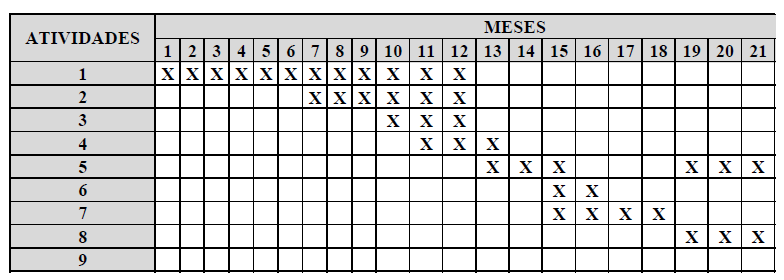
\includegraphics[scale=0.8]{cronograma}
\end{figure*}
\nocite{*}
\bibliographystyle{IEEEtran}
\bibliography{IEEEexample}

\end{document}
